\documentclass{article}[10pt]

\usepackage{fullpage}
\usepackage{parskip}
\usepackage{color}
\usepackage{listings}
\usepackage{amsmath}
\usepackage{graphicx}
\usepackage{caption}
\usepackage{subcaption}
\usepackage{wrapfig}
\usepackage{multirow}
\usepackage[compact]{titlesec}

\lstset{basicstyle=\ttfamily}
\lstset{keywordstyle=\ttfamily\bfseries}
\lstset{language=LISP}
\lstset{columns=fullflexible}

\begin{document}
\title{Program Synthesis for DNA Strand Displacement}
\author{Kendall Stewart, Anthony Ha, Martin Kellogg}
\date{\vspace{-5ex}}

\maketitle

\section{Introduction}

DNA computing seeks to leverage the chemical properties
of DNA molecules as a computational substrate.
From a medical perspective, DNA computing can enable the
construction of complex devices at a cellular scale for more precise
diagnostic tests or drug delivery. From a computer architecture perspective,
DNA is capable of performing massively parallel computations with very low
power consumption.

The feasibility of DNA computing was first demonstrated by encoding the
Hamiltonian Path Problem into DNA~\cite{adelman}. This encoding was constructed
by hand, but recent work has advanced DNA strand displacement reactions as a
primitive for DNA computation, because they can implement a wide
range of algorithms and devices, including boolean circuits~\cite{strands},
oscillators~\cite{dsd}, and neural networks~\cite{strandnn}.
However, strand displacement circuits can be difficult to reason
to reason about.

\section{Overview of Our Approach}

A formal semantics for strand displacement reactions is provided in the
description of DSD~\cite{dsd}, a programming language for specifying and
simulating DNA strand displacement circuits. Given a set of initial strand
species (reactants), DSD applies reduction rules to infer the intermediate and
final strand species (products), and creates a directed reaction graph with
edges between reactants and products, weighted by the rate of each reaction.
This graph, along with ordinary differential equations derived from the rates,
are used to simulate the strand displacement system.
Ignoring rates, the structure of the unweighted reaction graph encodes
conditions that are necessary (but not sufficient) for some product to have a
particular meaning. For instance, if all paths leading to a product include both
initial species $A$ and initial species $B$, the product could
represent $A \land B$.

We have implemented an interpreter for the semantics of DSD in
Rosette~\cite{rosette}. By writing predicates over reaction graphs, we can ask
Rosette's solver to fill in symbolic holes in DSD programs such that the outputs
have a particular meaning.  Our tool is able to able to discover a system
representing an AND gate that is equivalent to one designed by hand, and it is
also able to discover a system representing an OR gate that is smaller than a
common hand-designed system.

\section{Algorithms and Encodings}

\subsection{Syntactic Encoding}

The core syntactic unit of DSD is a \emph{domain}, which identifies
a unique sequence of DNA bases.  Identifiers ending
in a \lstinline{^} represent short (or \emph{toehold}) domains,
while all other identifiers represent long domains.
Individual bases in the sequence are arbitrary, but distinct identifiers must
map to non-interfering sequences.
Every domain has a \emph{complement}, which is denoted
with a \lstinline{*} after the identifier. A domain's complement is
the Watson-Crick complement of the underlying bases: \lstinline{A} and \lstinline{T}
are complementary, and \lstinline{C} and \lstinline{G} are complementary.  
For example, if \lstinline{1^} is \lstinline{ACTG}, then \lstinline{1^*}
is \lstinline{TGAC}.

DNA in solution can be either single or double-stranded.
In double-stranded DNA, a sequence of bases is bound with its complement.
In DSD, a \emph{strand} is a single-stranded sequence of zero or more domains, for
example \verb;<1 2 3>; (which can also be written as the rotationally symmetric
\verb;{3 2 1};).
A \emph{gate} is a double-stranded sequence of one or more domains,
along with optional single-stranded overhangs on the top and bottom of each
side, for example \verb;<1>{2}[3 4]{5}<6>;.
Two gates may also share an upper or lower strand. If \verb;G1; and \verb;G2;
are gates, upper-strand sharing is written \verb;G1::G2; and lower-strand
sharing is written \verb;G1:G2;.

Our encoding of DSD's syntactic constructs is straightforward.
Long domains are encoded as integers, while
short domains are integers wrapped in a \verb;toehold; struct.
The complement operation is also a \verb;struct;.
Sequences of domains are encoded as lists, and strands are lists
tagged with the type (upper, lower, or double-stranded). Gates
are a five-tuple of their constituent strands.
Example syntactic encodings are shown in Table~\ref{table:encoding-example}.

\begin{table}[h]
\centering
\begin{tabular}{|l|l|l|} \hline
Construct     & DSD Syntax    & Encoding                      \\ \hline
Long Domain   & \verb;0;      & \verb;0;                      \\ \hline
Toehold       & \verb;1^;     & \verb;(toehold 1);            \\ \hline
Complement    & \verb;1^*;    & \verb;(complement (toehold 1)); \\ \hline
Upper Strand  & \verb;<0 1^>; & \verb;(upper-strand (list 0 (toehold 1))); \\
\hline
Gate          & \verb;<1>{2^*}[3 4]{5}; &
\begin{lstlisting}
(gate
  (upper-strand (list 1))
  (lower-strand (list (complement (toehold 2))))
  (duplex-strand (list 3 4))
  (lower-strand (list 5))
  (upper-strand '()))
\end{lstlisting}
\\
\hline
\end{tabular}
\caption{Example of syntactic encoding.}
\label{table:encoding-example}
\end{table}

\subsection{Semantic Encoding}
\subsubsection{Reduction Rules}
DSD models the behavior of DNA strand displacement reactions with
\emph{reduction rules}---pattern-based rewrite rules
that model the conditions for and outcomes of a known reaction
involving DNA molecules. Reduction rules are also associated with
reaction rates, which model the kinetics of each chemical reaction.

The DSD specification refers to the set of reduction rules being used
as the level of \emph{semantic abstraction}, and defines four such levels.
More refined levels
use more rules, and produce more intermediate species. The
coarser abstractions use fewer rules (and merge some rules together),
thus eliding intermediate species.

Our encoding implements the coarsest semantic abstraction level,
the \emph{infinite} abstraction. This abstraction only has one
rule (rule RP) which describes binding interactions between a strand and a gate
that can lead to a strand displacement reaction (where a strand is
released from the gate). The infinite abstraction also allows for the strand
displacement reaction itself (rule RD)
to be merged into the RP reaction.
Rules RP and RD, and an outline of their merged encoding in Rosette, are shown in
Figure~\ref{figure:example-rule}. The outermost \verb;match*; expression
performs a purely syntactic match to check whether the species have
the correct type and bind their fields to variable names.
The inner \verb;match; and \verb;cond;
expressions discover if the domains of the input species satisfy
the requirements of the rule. The result is a \verb;reaction;,
(a 4-tuple containing the input strand and gate, and the
output strand and gate). The empty list in either output indicates
that the reaction does not produce that output; if the empty list
is in both outputs, it means that no reaction occurs.

\begin{figure}[h]
\centering
\begin{subfigure}[c]{0.35\textwidth}
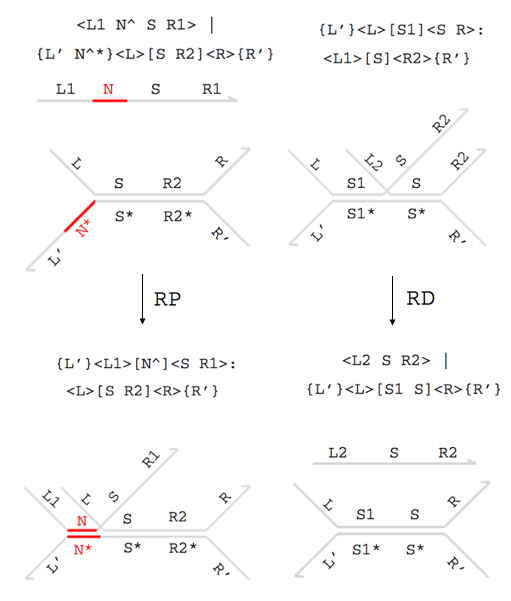
\includegraphics[width=\textwidth]{figures/rule-merge.png}
\end{subfigure}
~
\begin{subfigure}[c]{0.5\textwidth}
\begin{lstlisting}[basicstyle=\scriptsize\ttfamily]
(define (rule-rp strand-in gate-in)
  (match* (strand-in gate-in)
    [ ((upper-strand upper)
       (gate
        (upper-strand left-upper) (lower-strand left-lower)
        (duplex-strand duplex)
        (lower-strand right-lower) (upper-strand right-upper)))

      (match (toehold-search upper left-lower)
        ...
        ; matching toeholds
        [ (list ...)
          ; conditional merge with other rules
          (cond
            ...
            ; strand displacement
            [ ...
               (reaction
                strand-in gate-in
                (upper-strand ...)
                (gate ...)) ]) ]) ]

    [ (_ _) (reaction strand-in gate-in '() '()) ]))
\end{lstlisting}
\end{subfigure}
\caption{
DSD rules RP and RD, and their encoding as a merged rule, \lstinline{rule-rp} in
Rosette.  On the left, all identifiers (\lstinline{S}, \lstinline{R2}, etc.)
represent domain concatenations (lists of domains), except for \lstinline{N},
which represents a single toehold domain.
}
\label{figure:example-rule}
\end{figure}

\subsubsection{Reaction Graphs}

Given a set of input species, DSD computes a \emph{reaction graph} by applying
reduction rules to exhaustion (until no new species are produced). The vertices
of the graph are individual species, and edges between species indicate
reactions, weighted by the reaction rate. Reactions that require two species
join the edges from the two input species into a single edge leading to the
output. Reactions may also be reversible, indicated by a back edge from the
outputs to the inputs.

This graph
and its properties constitute the \emph{meaning} of a DSD program.
The reactions and their corresponding weights can be used to simulate
the progress of the system over time. At a coarser level of abstraction
(i.e. ignoring rates) the structure of the graph encodes whether or not
it can have a particular meaning. The reaction
graph for a system representing an AND gate is shown in
Figure~\ref{figure:and-gate}. This system represents an AND gate
because all reactions that produce the strand \verb;<2 3>;
require (either directly or indirectly) both of the inputs.
We can write this requirement as a predicate in first-order logic, as
follows. Given a reaction graph $g$, and input strands $i_1$ and $i_2$:
\begin{equation}
\mathrm{isAndSystem}(g, i_1, i_2) =
\exists x \in \mathrm{strands}(g)\ .\ 
\forall p \in \mathrm{parents}_g(x)\ .\ 
\mathrm{requires}_g(p, i_1) \land \mathrm{requires}_g(p, i_2)
\label{eq:and-sys}
\end{equation}

Here, the function $\mathrm{strands}(g)$ returns the set of single strands in
the reaction graph $g$, and the function $\mathrm{parents}_g(x)$ returns
the set of parent reactions of the strand $x$ in graph $g$. The predicate 
$\mathrm{requires}_g(p,i)$ is true if the reaction $p$ cannot happen
(either directly or indirectly) without the strand $i$ in graph $g$.
It is easy to see that this predicate is satisfied for the graph in
Figure~\ref{figure:and-gate}.

\begin{figure}
\centering
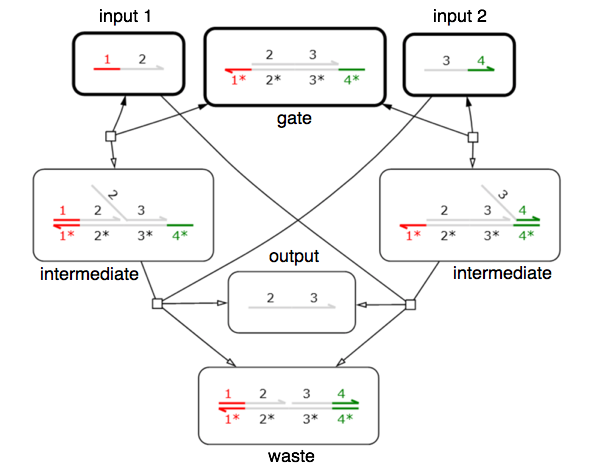
\includegraphics[width=0.5\textwidth]{figures/and-gate.png}
\caption{
The result of compiling the DSD program
\texttt{(<1\^{} 2>|<3 4\^{}>|\{1\^{}*\}[2 3]\{4\^{}*\})}
}
\label{figure:and-gate}
\end{figure}

\subsection{Solver-Aided Queries}
\subsubsection{``Synthesizing" DSD Programs}
Our goal is to apply a first-order predicate such as Equation~\ref{eq:and-sys}
to a reaction graph where the identity of one or more domains in the input
species is left symbolic, and then ask a solver to find bindings for the
symbolic variables such that the predicate is satisfied. However,
to compile a reaction graph, DSD requires applying
reduction rules until no new species are generated; this poses a problem
for symbolic execution, because the termination of this algorithm
depends on the identity of the species, and termination cannot be
predicated on symbolic values. Therefore, we finitize the computation
of the reaction graph by only considering a small number of possible
reactions: the reactions between the initial species, and between
the products of those reactions and the initial species. The
resulting reaction graph will have a concrete size for a given
number of input strands and gates. This finitization
is still powerful enough to reason about small systems such as the one
depicted in Figure~\ref{figure:and-gate}, where no reactions on the
paths to the output are only between intermediate species.

Since all reaction graphs are of a finite size and concrete shape,
writing a predicate such as the one in Equation~\ref{eq:and-sys} is
simple: sets are represented as lists, and we use Rosette's \verb;ormap; for
existential quantification and \verb;andmap; for universal quantification.
Applying this predicate to a reaction graph with symbolic inputs results
in a formula that can be passed to Rosette's \verb;solve; procedure.
Strictly speaking, this process is not inductive synthesis, because it
does not require universal quantification over inputs---we are simply
asking the solver to fill in a finite number of domain ``holes" such that the
predicate is satisfied.

\subsubsection{Verified Continuous Integration}
As we were working on writing reduction rules, we were originally
checking our code with traditional \emph{ad hoc} testing. But,
since we were working in Rosette, we were able to use the \verb;verify;
form to check semantic properties of the rules and find bugs in the
form of counterexamples. These verified tests were also used as regression
tests, and run by our CI server on each commit to help ensure that our code
stayed correct.

\section{Results}

\subsection{Case Study: AND and OR gates}

We tested our system with two sketches and predicates: isAndSystem
(Equation~\ref{eq:and-sys}) and isOrSystem. isOrSystem
requires the graph to have an output
with at least two parent reactions, each of which exclusively
require one of the inputs. A system satisfying this predicate creates the output
if either input is present.
The sketches are inspired by the structure of
known AND and OR gates. The known AND gate is shown in
Figure~\ref{figure:and-gate}. The known OR gate is from
a set of slides by UW CSE Professor Georg Seelig \cite{seelig}.

The results of these queries are shown in Table~\ref{table:results}.
The solver performs as expected on the AND gate: the resulting reaction graph
is nearly identical to the hand-designed AND gate (except that solver decided
to use the same domain twice for the output rather than two different domains).
The OR gate on its original sketch is more interesting: the solution has holes,
which allows two of the gates to be collapsed into one.
An even simpler solution is found if we ask the solver
to implement an OR gate with the smaller sketch intended for the AND gate.
The hand-designed OR gate from Professor Seelig's slides is actually a motif
that allows for potentially unbounded fan-in; however, the solver
finds an OR gate that is optimized for just two inputs. This
is an encouraging result: while abstract motifs are easier for
humans to reason about, a solver may find optimizations
for special cases that are more efficient but harder to discover.

\begin{table}
\centering
\begin{tabular}{|l|l|l|l|l|}\hline
Sketch   & Graph Size & Predicate & Result & Total Time \\ \hline
\begin{lstlisting}[basicstyle=\scriptsize\ttfamily]
(<?? ??>
|<?? ??>
|{??}[?? ??]{??}
)
\end{lstlisting}
&
28
&
isAndSystem
&
\begin{lstlisting}[basicstyle=\scriptsize\ttfamily]
(<5^ 2>
|<2 5^>
|{5^*}[2 2]{5^*}
)
\end{lstlisting}
&
3 seconds
\\ \hline
''
&
''
&
isOrSystem
&
\begin{lstlisting}[basicstyle=\scriptsize\ttfamily]
(<8^ 7^>
|<7^ 8^>
|{7^*}[8^ 8^]{7^*}
)
\end{lstlisting}
&
3.4 seconds
\\ \hline
\begin{lstlisting}[basicstyle=\scriptsize\ttfamily]
(<?? ?? ?? ??>
|<?? ?? ?? ??>
|{??}[?? ??]<?? ??>
|{??}[?? ??]<?? ??>
|{??}[?? ??]<?? ??>
)
\end{lstlisting}
&
132
&
isOrSystem
&
\begin{lstlisting}[basicstyle=\scriptsize\ttfamily]
(<7^ ?? 5^ 5^>
|<?? 5^ 6^ ??>
|{5^*}[6^ 6^]<5^ ??^>
|{5^*}[6^ 6^]<?? ??>
|{5^*}[5^ 6^]<5^ ??>
)
\end{lstlisting}
&
54 seconds
\\ \hline
''
&
''
&
isAndSystem
&
\verb;(unsat);
&
290 seconds
\\ \hline
\end{tabular}
\caption{Summary of results for two sketches and predicates.}
\label{table:results}
\end{table}

\subsection{Limitations and Future Work}
The extreme finitization of the compilation process limits the complexity
of the reaction networks our system can reason about. The core problem is
that we must consider all possible interactions between all possible
intermediate products, which grows exponentially with the number of steps away
from the initial species. A possible solution
is a domain-specific structuring of the search space (a la metasketches
\cite{metasketches}), to prioritize portions that are more likely to be
fruitful. Moreover, our abstraction is extremely coarse, which means that the
solutions the solver generates may seem weak to a domain scientist.
Metasketches could again help here by providing a domain-specific
cost function to help guide the search.

We believe the first step towards publishing this work would be to
consult a domain scientist that works with DNA strand displacement,
and have them provide a motivating and interesting problem to work
towards (more so than the toy AND and OR gates explored here).
If this tool can solve problems that domain scientists find difficult
to reason about, it could have quite an impact in the DNA computing
community.

\section{Teamwork}

Our initial meetings sketched out the architecture of the interpreter and our
syntactic encoding, in which we all had an equal role. Subsequently we divided
tasks amongst the team members: Kendall wrote the reduction rules, the graph
compilation procedure, the semantic graph predicates, and the demo. Anthony
wrote the DSD parser and pretty-printer, a reaction graph visualizer (for an
early graph representation, now not used), and also wrote procedures to
manipulate species (rotation, complement, etc). These were intended to be
part of a normalization procedure specified by DSD. This procedure did not end
up being used in our final simplified algorithm, but could be useful in future
work.  Martin focused on verification and testing of our code, including writing
solver-aided unit tests and the deployment of a test infrastructure using
continuous integration. Kendall and Martin wrote this report.

\section{Course Topics}

This project is built on top of Rosette, a solver-aided language, and makes
use of Rosette's ability to perform angelic execution and bounded verification.
In particular, the symbolic holes in the input species are angelic choices,
and the verified tests check whether a property is valid by checking if its
negation is unsatisfiable. We did not encounter any roadblocks that could
not be answered by course material, and in fact the lecture on Rosette
precipitated some useful insights for how to make the symbolic execution
efficient (e.g., try to ensure that objects on the heap rarely change their
shape).


\begin{thebibliography}{9}

\bibitem{adelman}
L. M. Adleman,
“Molecular computation of solutions to combinatorial problems,”
Science, vol. 266, no. 5187, pp. 1021–1024, Nov. 1994.

\bibitem{strands}
D. Y. Zhang and G. Seelig,
“Dynamic DNA nanotechnology using strand-displacement reactions,”
Nature Chemistry, vol. 3, no. 2, pp. 103–113, Feb. 2011.

\bibitem{dsd}
M. R. Lakin, S. Youssef, L. Cardelli, and A. Phillips,
“Abstractions for DNA circuit design,”
Journal of The Royal Society Interface, vol. 9, no. 68, Jul. 2011.

\bibitem{strandnn}
L. Qian, E. Winfree, and J. Bruck, “Neural network computation with DNA strand
displacement cascades,” Nature, vol. 475, no. 7356, pp. 368–372, Jul. 2011.

\bibitem{rosette}
 E. Torlak and R. Bodik, “A lightweight symbolic virtual machine for solver-aided host languages,” Programming Language Design and Implementation (PLDI), vol. 49, no. 6, pp. 530-541, 2014.

\bibitem{seelig}
G. Seeling, ``Logic circuits with DNA
strand displacement". Slides for CSE590: Molecular Programming and
Neural Computation. Presented Jan 24th, 2014.

\bibitem{metasketches}
J. Bornholt, E. Torlak, D. Grossman, and L. Ceze, “Optimizing Synthesis with
Metasketches,” POPL, 2016.

\end{thebibliography}

\end{document}
